\documentclass[../dissertation.tex]{subfiles}
 
\begin{document}

\section{Experiment 1}

\subsection{Methods}
\subsubsection{Participants}
\subsubsection{Category Learning Task}
	This task measures learning of dense and sparse categories and is based off of a paradigm from previous research \citep{Kloos2008}. Participants learn novel categories of items in four possible conditions in a 2 x 2 design. The first manipulation is learning type (supervised vs. unsupervised). In \textit{supervised} learning, participants learn the categories by being instructed on the relevant features (e.g., “All friendly aliens have big noses.”). Images of the relevant features are provided along with the descriptions. In \textit{unsupervised} learning, participants learn the categories by viewing sixteen instances of the category. \par
	The second manipulation is category type (sparse vs. dense). Category type is measured by statistical density, which ranges from zero (where all features vary freely) to one (where all features co-occur perfectly). It is based on a comparison between within- and between-category entropy \citep{Sloutsky2010}. All categories in this experiment have seven dimensions. The \textit{sparse} categories cohere on a single dimension, while the other dimensions vary freely (density = .25). In contrast, the \textit{dense} categories cohere on six of the seven dimensions (density = .75). The seventh dimension is allowed to vary freely. For more details on how density was calculated, see Appendix A. Stimuli for each of the four blocks are different. See Fig. \ref{sloutskymanip} for examples of the experimental manipulations. \par
\begin{figure}[htp]
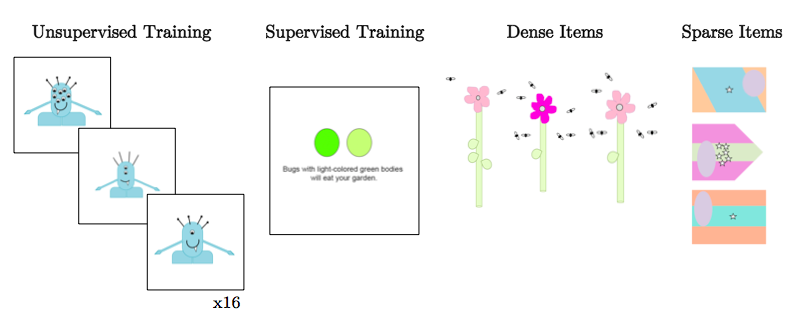
\includegraphics[width=\textwidth]{manipulations}
\caption{Examples of learning type and category type manipulations for category learning experiment.}
\vspace{-10pt}
\label{sloutskymanip}
\end{figure}

\begin{wraptable}[11]{r}{0.6\linewidth}
\caption{Block orders for statistical density task}
\vspace{-10pt}
\begin{center}
\begin{tabular}{ c|c|c|c } 
 \hline 
 Effect & Group & Block 1 & Block 2 \\ 
 \hline
 \multirow{2}{*}{1} & 1 & Unsupervised-dense & Supervised-sparse \\ 
 & 2 & Supervised-sparse & Unsupervised-dense \\ 
 \hline
  \multirow{2}{*}{2} & 3 & Unsupervised-dense & Supervised-dense \\ 
 & 4 & Supervised-dense & Unsupervised-dense \\
 \hline 
  \multirow{2}{*}{3} & 5 & Unsupervised-sparse & Supervised-sparse \\ 
 & 6 & Supervised-sparse & Unsupervised-sparse \\ 
 \hline
\end{tabular}
\end{center}
\label{exp1order}
\end{wraptable} 
	This task is within-subjects. Based on the group they were placed into, participants will complete two of the four possible learning-category type combinations. In this experiment, I tested three main order effects. First, I tested order effects for the matching conditions (unsupervised-dense and supervised-sparse).The second order effect used unsupervised-dense and supervised-dense blocks. Finally, the third order effect tested the same sparse stimuli, testing unsupervised-dense and supervised-sparse blocks. This design led to six possible order groups that each participant could be placed into. See Table \ref{exp1order} for a summary. \par
 In each block, participants were introduced to the task through a short cover story. They were told to learn which items go with a certain property (e.g., which aliens are friendly). Crucially, no labels were attached to the categories (e.g., some aliens are Ziblets). Then, participants completed a training block (either supervised or unsupervised). After training, participants completed 40 test trials (16 target, 16 distractor, 8 catch), following the design of \citet{Kloos2008} . In each trial, participants saw a single item and used the keyboard to indicate whether the item matched the category they had just learned (e.g., if the alien is friendly). Catch items look significantly different than both the target and competing categories, so participants should always reject them as members of the learned category. This experiment was presented using PsychoPy v.1.84.2 \citep{Peirce2007}. \par

\subsubsection{Behavioral Measures}
	I used multiple assessments to test participants' language ability. The choice of assessments was based on the epiSLI criteria for language impairment \citep{Tomblin1996}, which includes comprehension, expression, vocabulary, grammar, and narrative. I adapted these requirements from a kindergarten population to a college-aged population. The epiSLI criteria have been shown to be robust for diagnosis of specific language impairment (SLI). In addition, other studies of language impairment more broadly have adapted a similar multidimensional approach to measuring language ability, sometimes including measures of phonological skills \citep{Catts2006}. Thus, using assessments that the many domains of language outlined in epiSLI criteria will allow me to get a fuller picture of individual differences in language ability. See Table \ref{slitable} for a summary of the assessments and which domains of the epiSLI criteria they cover. The specific tests used in this experiment are detailed below. \par
	\textbf{Test of word reading efficiency (TOWRE) phonemic decoding subtest.} TOWRE is a test of nonword fluency \citep{Torgesen1992}. This test is a part of the comprehension aspect of epiSLI, since the comprehension measure is reading-based. In the TOWRE, individuals have 45 seconds to read as many nonwords as possible. The nonwords become longer and more difficult as the list goes on. \par
	\textbf{Woodcock Johnson-III word attack (WA) subtest.} This task measures nonword decoding ability \citep{Woodcock2001}. Like the TOWRE, it is helpful for measuring the comprehension aspect of epiSLI. However, while the TOWRE measures word fluency, this task measures decoding accuracy. Participants read a list of nonwords out loud at their own pace. \par
	\textbf{Computerized reading comprehension.} This test covers the comprehension and narrative aspects of epiSLI. This computerized reading comprehension test is based on the Kaufman Test of Educational Achievement (KTEA) reading comprehension subtest \citep{Kaufman2004}. To create this test, I copied the passages and questions contained in the KTEA reading comprehension subtest into E-Prime \citep{schneider2002prime} for presentation on a computer. I created multiple choice answers for the KTEA questions that did not already have them. In this task, participants read short expository and narrative texts and answered multiple-choice comprehension questions about them. Some questions are literal, while others require participants to make an inference. Because this task is a modified version of the KTEA, I use raw scores in analysis rather than standardized scores based on the KTEA norms. \par
	\textbf{Nelson-Denny vocabulary subtest.} The Nelson-Denny vocabulary sub-test is a written assessment of vocabulary \citep{Brown1981}. This test covers the vocabulary aspect of epiSLI. This test has been used in multiple studies of college-aged adults and provides sufficient variability for individual difference investigations in this population \citetext{e.g., \citealt{Boudewyn2015}; \citealt{Stafura2014}}. In this test, participants are asked to choose the word closest to a target vocabulary word. \par
	\textbf{Clinical Evaluation of Language Fundamentals recalling sentences subtest.} I will use the recalling sentences subtest from the Clinical Evaluation of Language Fundamentals \citetext{CELF; \citealt{BSemel2006}; \citealt{Stafura2014}}. This test covers the grammar and expression aspects of epiSLI. In this subtest, participants hear sentences and are asked to repeat them. Scoring is based on how many errors the participant makes in their repetition.  \par
	Finally, I used Set II of Raven's Advanced Matrices to measure nonverbal IQ \citep{Raven1998}. In this task, participants see a grid containing eight images and an empty space. The images are arranged in the grid according to some rule or rules. Participants must choose one of eight additional images that fits in the empty space.

\begin{table}[H]
\caption{Assessments of language and their corresponding epiSLI domains.}
\vspace{-10pt}
\begin{center}
\begin{tabular}{ c|c } 
 \hline 
 Test & epiSLI Criteria \\ 
 \hline
 TOWRE & \multirow{2}{*}{Comprehension (decoding aspect)}\\ 
 WA & \\ 
 Computerized Reading Comprehension & Comprehension, narrative \\
 ND Vocab & Vocabulary \\ 
 CELF RS & Grammar, expression \\ 
 \hline
\end{tabular}
\end{center}
\label{slitable}
\end{table}


\subsection{Procedure}
	Each participant completed the category learning task as well as all of the behavioral measures. TOWRE, WA, and CELF were audio-recorded to allow for offline scoring. To allow multiple subjects to be run in a single timeslot, some participants received tasks they could complete on their own (category learning, ND, Computerized reading comprehension, Raven's) first while others completed tasks with the experimenter first (WA, CELF, TOWRE). All together, the seven tasks took approximately one hour.
	
\subsection{Results}

\subsection{Discussion}

\end{document}

